% ETAPS 2027 submission draft for TACAS (18 pages excluding references)
% or iFS (16 pages plus 2 pages of references). Both venues require LNCS and
% double-blind review for regular research papers.
\documentclass[runningheads]{llncs}

\usepackage[T1]{fontenc}
\usepackage{amsmath,amssymb}
\usepackage{booktabs}
\usepackage{graphicx}
\usepackage{placeins}
\usepackage[hidelinks]{hyperref}
\usepackage{alloy}
\usepackage{beramono}

% Keep this true for double-blind submission; set it false for camera-ready.
\newif\ifanonymous
\anonymoustrue

\begin{document}

\title{Symbolic Synthesis of Distinguishing Test Batches for Specification Narrowing}
\titlerunning{Synthesis of Distinguishing Test Batches}

\ifanonymous
  \author{Anonymous Authors}
  \authorrunning{Anonymous Authors}
  \institute{}
\else
  \author{Alcino Cunha\inst{1} \and Nuno Macedo\inst{1}}
  \authorrunning{A. Cunha and N. Macedo}
  \institute{INESC TEC and Universidade do Minho, Braga, Portugal\\
    \email{alcino@di.uminho.pt, nmacedo@di.uminho.pt}}
\fi

\maketitle

\begin{abstract}
Weak or ambiguous requirements can give rise to several non-equivalent formal
specifications. A domain expert can narrow the candidates by classifying
concrete instances or traces on which they disagree. We study the symbolic
synthesis of complete distinguishing test batches. Such batches support
asynchronous and parallel review, predictable workload, auditability, and
reproducibility, yet adaptive presentation can stop as soon as one candidate
remains. We propose four symbolic constructions. Two tree-guided methods
recursively partition the candidates using balanced MaxSAT or feasibility-only
SAT and reuse tests across branches. Two cover-based methods minimize batch
cardinality globally, either by joint MaxSAT synthesis or by enumerating
attainable separation patterns before solving an explicit cover. All four use
the same adaptive presentation policy. Our experiments show that balanced
batches essentially attain the unrestricted binary-tree lower bound on the
number of classifications. Recursive SAT is markedly more robust with
virtually the same classification cost, while exact cover-based methods
substantially reduce artifact size without a material classification penalty.
Synthesizing a complete batch requires more time than synthesizing only the
tests needed along a single narrowing path, but provides a stable, reusable
artifact. Overall, the choice among methods is driven chiefly by synthesis
robustness and artifact size, not classification cost.

\keywords{Specification narrowing \and Symbolic test synthesis \and MaxSAT
  \and Alloy \and Temporal relational logic}
\end{abstract}

\section{Introduction}
\label{sec:introduction}

Developing a formal model may require choosing among alternative
specifications because weak or ambiguous requirements admit multiple
interpretations. Candidates may be written by different experts or produced
automatically. Program synthesis and repair, for example, may return several
artifacts consistent with incomplete input/output
examples~\cite{shriver2017end}; related techniques synthesize temporal
specifications from examples~\cite{gavran2020interactive,zhang2025constrained}
and repair relational
specifications~\cite{wang2019arepair,brida2021beafix,gutierrez2022icebar,cerqueira2022timely}.
More recently, LLMs have been used to generate formal specifications from
natural language, a process known as
\emph{autoformalization}~\cite{weng2025autoformalization,mendoza2026automating}.
Neither consistency with available examples nor syntactic proximity to a
faulty original specification establishes which candidate captures the
intended requirement. Moreover, because autoformalization starts from
potentially ambiguous natural-language requirements, it does not itself provide
an independent semantic oracle. Choosing among the candidates may therefore
require a domain expert unfamiliar with the formal notation, for whom comparing
dozens of formulas is infeasible.

To identify the intended candidate, we can obtain additional semantic evidence
from a domain expert's judgment of a concrete test---an instance or execution
trace---on which candidates disagree. Classifying the test as desirable or
undesirable eliminates candidates that answer differently.
Existing narrowing approaches synthesize tests \emph{online}, using each
classification to choose the next test for the remaining
candidates~\cite{shriver2017end,gavran2020interactive,mendoza2026automating}.
This paper focuses instead on complete distinguishing \emph{batches} synthesized
before classification. A fixed batch supports asynchronous and parallel
review, comparable and auditable judgments, a predictable upper bound on
workload, and the reproduction or subsequent revision of decisions. However,
when
used for specification narrowing, it need not be reviewed in full: after each
answer, the tool can present the unused test that
best partitions the remaining candidates and stop once at most one remains.

We study four ways to construct such batches, organized by how they establish
distinguishability. Two are \emph{tree-guided}: they recursively split a set of
remaining candidates and explore both outcomes before interaction. Two are
\emph{cover-based}: they instead select tests that collectively separate every
candidate pair without constructing a decision tree. In either family, a
method may target balanced partitions, minimum cardinality, or inexpensive and
reliable synthesis. These objectives need not coincide. Our novelty lies not in distinguishing scenarios themselves, but in
synthesizing a complete reusable batch directly from an implicit symbolic test
space and comparing tree-guided and globally cardinality-minimal constructions
under a common adaptive presentation policy.

We ask how tree-guided and cover-based symbolic constructions differ in batch
cardinality and synthesis scalability, whether these differences materially
affect classification cost, and how much additional synthesis time complete
precomputation requires relative to always-online balanced synthesis.
When used for specification narrowing, every resulting batch follows the same
adaptive policy: present the stored test that most evenly divides the remaining
candidates. This selection is cheap because it only ranks already synthesized
tests. We compare how well the constructed batches support balanced adaptive
presentation, how much exact cardinality minimization compresses the artifact,
and how reliably the methods produce a complete batch.

We formalize distinguishing batches and instantiate four constructions for
Alloy's temporal relational logic~\cite{jackson2012software,jackson2019alloy}.
The two tree-guided methods both reuse tests across candidate subsets. Balanced
MaxSAT optimizes the feasible split whenever no stored test is already optimal;
Recursive SAT uses only inexpensive feasibility queries. The two cover-based
methods are exact: symbolic MaxSAT jointly synthesizes a cardinality-minimum
batch, while separation-pattern enumeration materializes the attainable
partitions before solving the resulting Minimum Test Set
problem~\cite{GareyJohnson,moret1985minimizing}. The implementation uses
AlloyMax~\cite{zhang2021alloymax} and supports both
structural instances and bounded temporal traces through an explicit lasso
encoding.

Across 196 configurations derived from 28 requirements in three models,
the balanced batch lies within 0.004 classifications of the unrestricted
binary-tree lower bound, so an optimal always-online policy can save at most
0.004 classifications on average. Synthesizing only the observed online path
reduces paired median synthesis time from 1.65 to 0.82 seconds. Recursive
batches require 4.18 classifications against 4.15 for balanced batches and tie
on 66\% of paths. On 151 jointly completed configurations, exact synthesis
reduces the balanced batch from 7.36 to 5.17 tests on average. Recursive
synthesis completes every configuration, whereas the other three methods
exhibit timeouts.
A temporal replication preserved the classification and cardinality trends but
reversed the cover methods' completion ordering: Enumeration completed 31 of
32 configurations, against 9 for Exact MaxSAT.

This paper contributes:
\begin{itemize}
  \item a formalization of adaptively presented distinguishing batches that
    separates classification cost, synthesis cost, and batch cardinality;
  \item Balanced MaxSAT and Recursive SAT, two tree-guided constructions that
    reuse tests across branches;
  \item Exact MaxSAT and separation-pattern enumeration, two cover-based
    exact methods that minimize batch cardinality; and
  \item an exhaustive comparison of the four methods across classification
    cost, artifact size, synthesis cost, and scalability.
\end{itemize}

\section{Running Example}
\label{sec:example}


\begin{figure}[t]
\begin{alloy}[basicstyle=\scriptsize\ttfamily]
// domain model
sig Person { teaches, enrolled : set Course, workson : set Project }
sig Professor, Student in Person {}
sig Course { projects : set Project }
sig Project {}
fact Assumptions {
  all c : Course | some teaches.c
  teaches.Course in Professor and enrolled.Course in Student
  all p : Project | lone projects.p
  all p : Person | no (p.teaches & p.enrolled)
  all p : Person | p.workson in p.enrolled.projects
}
// candidate specifications
pred Spec1 { all p : Professor | 
  no (p.teaches & (Professor - p).enrolled)
}
pred Spec2 { all p, q : Professor |
  (some (p.enrolled & q.enrolled) and p != q) implies no (p.teaches & q.enrolled)
}
pred Spec3 { all p, q : Professor |
  (some (p.teaches & q.teaches) and p != q) implies no (p.teaches & q.enrolled)
}
pred Spec4 { all p : Professor |
  let colleagues = { q : Person | q != p and some (p.workson & q.workson) } |
    no (p.teaches & colleagues.enrolled)
}
pred Spec5 { all p : Professor |
  let colleagues = { q : Professor | q != p and some (p.workson & q.workson) } |
    no (p.teaches & colleagues.enrolled)
}
pred Spec6 { all p, q : Professor |
  (p != q and some ((p.teaches.~enrolled) & (q.teaches.~enrolled))) implies
  no (p.teaches & q.enrolled)
}
\end{alloy}
\caption{University-course domain model and six non-equivalent candidate specifications returned by GPT-5.2 for a new requirement (analysis commands omitted).}
\label{fig:courses-model}
\end{figure}

Figure~\ref{fig:courses-model} shows an Alloy model of university courses.
Its signatures and fields represent people, courses, projects, teaching,
enrollment, and project work; the facts constrain their admissible
relationships.
Suppose we want to formalize the new requirement ``a professor cannot teach colleagues''. This requirement is ambiguous
because it does not define a colleague. Asked to formalize it, GPT-5.2 returned
nine predicates; Fig.~\ref{fig:courses-model} shows the six that are
non-equivalent under the facts. They interpret colleagues as every other
professor (\a{Spec1}),
professors enrolled in a common course (\a{Spec2}), professors who co-teach a
course (\a{Spec3}), people who work on a common project (\a{Spec4}), professors
who work on a common project (\a{Spec5}), and professors who have a student in
common (\a{Spec6}). Their similarity makes direct comparison difficult. We
assume \a{Spec3} is intended and abbreviate \a{Spec}$i$ as $S_i$.

\paragraph{Minimum cover batch}
A cover-based method selects tests that collectively separate every candidate
pair without following a particular decision tree. The two cover-based methods
use different construction procedures, but both minimize the resulting batch
cardinality. Table~\ref{tab:batch-matrix} shows one possible batch. A check
mark denotes satisfaction; its six distinct columns distinguish all candidates.
Two binary tests encode at most four patterns, so three is
cardinality-minimum for this candidate set.

\begin{table}[t]
\centering
\caption{A minimum three-test batch and its adaptive use for \a{Spec3}.}
\label{tab:batch-matrix}
\small
\setlength{\tabcolsep}{5pt}
\begin{tabular}{lcccccc l}
\toprule
 & $S_1$ & $S_2$ & $S_3$ & $S_4$ & $S_5$ & $S_6$ & Adaptive use \\
\midrule
$T_1$ & -- & \checkmark & \checkmark & -- & \checkmark & -- & 1: desirable \\
$T_2$ & -- & \checkmark & -- & \checkmark & \checkmark & \checkmark & 2: undesirable \\
$T_3$ & -- & -- & \checkmark & \checkmark & \checkmark & -- & not requested \\
\bottomrule
\end{tabular}
\end{table}

For any distinguishing batch, a natural adaptive presentation policy chooses
the unused test that most evenly splits the remaining candidates. This step is
cheaper than synthesis because it only ranks stored tests, although it cannot
select a more balanced feasible test that happens to be omitted from the batch.
Here, $T_1$ can be chosen first; its desirable answer leaves
$\{S_2,S_3,S_5\}$. Test $T_2$ then isolates $S_3$; an undesirable answer
therefore selects $S_3$. Thus, the expert classifies only two of the three
precomputed tests. Figure~\ref{fig:courses-test2} depicts $T_2$: one professor
co-teaches a course with another professor and teaches a course in which that
colleague is enrolled, precisely
the situation rejected by \a{Spec3}. The expert can judge this concrete
scenario without reading the predicates.

\begin{figure}[t]
  \centering
  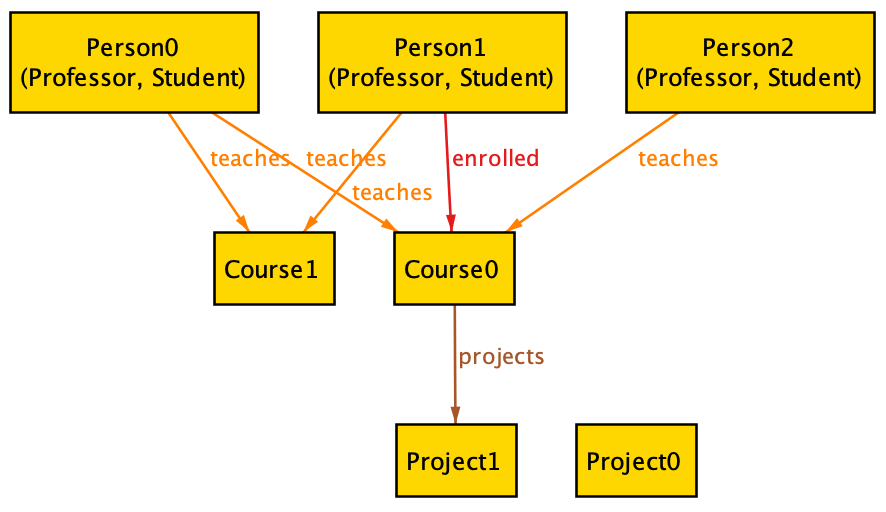
\includegraphics[width=.45\textwidth]{instance2.png}
  \caption{The decisive test $T_2$, visualized as an Alloy instance.}
  \label{fig:courses-test2}
\end{figure}

\paragraph{Tree-guided batches}
The tree-guided methods instead construct a decision tree by recursively
exploring both outcomes before interaction. On this example at scope~3,
Balanced MaxSAT reuses one test across the five internal tree nodes, stores four
distinct tests, and identifies $S_3$ after two classifications. Recursive SAT
stores five tests and requires three classifications. For comparison, Exact
MaxSAT and separation-pattern enumeration both produce cardinality-minimum
three-test batches, but their respective batches require three and two
classifications. Alternative minimum batches and balanced ties may change a
particular path. The example therefore illustrates that batch cardinality and
classification cost are distinct objectives, and motivates evaluating both
alongside synthesis effort.

\section{Distinguishing Test Batches}
\label{sec:problem}

We now formalize batch-based narrowing independently of Alloy. The formulation
requires only a finite set of feasible tests and the ability to decide whether
each candidate accepts a test. Section~\ref{sec:synthesis} then gives symbolic
batch constructions, and Section~\ref{sec:implementation} instantiates them for
Alloy.

\subsection{Candidates, Tests, and Classifications}

Let $F=\{\phi_1,\ldots,\phi_N\}$ be a set of candidate specifications over a
common vocabulary, and let $\mathcal{I}$ be the finite set of tests admitted by
the background theory and analysis bounds. A test may be a static instance or
an execution trace. Two candidates are distinguishable within the bounds if
some feasible test satisfies exactly one of them. We assume throughout that
the candidates are pairwise distinguishable. If no such test exists for a
pair, those two candidates agree on all admissible tests and cannot be
distinguished by test classification at the chosen bounds.

A classification history is a sequence
$H=\langle I_1^{c_1},\ldots,I_k^{c_k}\rangle$, where
$c_j\in\{+,-\}$, with $+$ denoting desirable and $-$ undesirable. The
candidates consistent with that history are
\[
  C(H)=\{\phi\in F \mid
    I\models\phi \text{ for every } I^+\text{ in }H,\;
    I\not\models\phi \text{ for every } I^-\text{ in }H\}.
\]
Narrowing is complete when $|C(H)|\leq 1$. The set $C(H)$ can be empty when
the complete set of judgments matches no candidate.

For example, the adaptive use of Table~\ref{tab:batch-matrix} produces the
history $\langle T_1^+,T_2^-\rangle$ and the successive candidate sets
\[
  F \xrightarrow{T_1^+} \{S_2,S_3,S_5\}
    \xrightarrow{T_2^-} \{S_3\}.
\]
Thus, that classification history narrows the candidates to $S_3$.

For $C\subseteq F$, let
\[
  C_+(I)=\{\phi\in C\mid I\models\phi\},\qquad
  C_-(I)=\{\phi\in C\mid I\not\models\phi\}.
\]
We say that $I$ \emph{splits} $C$ when both $C_+(I)$ and $C_-(I)$ are
nonempty. Pairwise distinguishability ensures that every $C$ with $|C|>1$
has a feasible splitting test.

\subsection{Batches and Adaptive Presentation}

A batch must contain enough semantic evidence to separate every pair of
candidates.

\begin{definition}
A \emph{distinguishing batch} for $F$ is a finite set
$T\subseteq\mathcal{I}$ such that, for every two distinct candidates
$\phi_i,\phi_j\in F$, some $I\in T$ satisfies exactly one of them. A
distinguishing batch is \emph{cardinality-minimum} if no smaller such batch
exists.
\end{definition}

Classifying every test in $T$ leaves at most one consistent candidate. A batch
need not, however, be presented in full or in a fixed order. Let $C$ be the
current candidate set and $R\subseteq T$ the tests not yet classified. An
adaptive presentation policy $\rho$ maps every reachable state $(C,R)$ with
$|C|>1$ to a test $\rho(C,R)\in R$ that splits $C$. If the expert returns
$c\in\{+,-\}$ for $I=\rho(C,R)$, the next state is
\[
  \bigl(C_c(I),R\setminus\{I\}\bigr).
\]
A suitable test always exists: any two candidates in $C$ are distinguished by
some member of $T$, and a previously classified test cannot distinguish
candidates that remain consistent with its answer.

Consider an intended candidate $\phi\in F$ as an \emph{oracle}, answering
positively exactly when $I\models\phi$. The classification cost
$\mathcal{C}_\rho(F,T,\phi)$ is the number of tests requested before at most one
candidate remains. For $N>1$,
\[
  1\leq \mathcal{C}_\rho(F,T,\phi)
  \leq\min\{|T|,N-1\}.
\]
In our experiments, $\rho$ greedily chooses the stored test that minimizes
\[
  b_C(I)=\max\{|C_+(I)|,|C_-(I)|\},
\]
with deterministic tie-breaking. This aims for a short decision path but only
ranks tests already synthesized in the batch.

\subsection{Tree-Guided and Cover-Based Batches}

A tree-guided constructor explores an implicit binary decision tree. At each
non-singleton candidate set $C$, it chooses a feasible test that splits $C$ and
recursively explores both outcomes. Tests generated for one node are retained
and may label later nodes, including nodes on another branch. Both our balanced
and recursive methods follow this scheme: balanced minimizes $b_C(I)$, whereas
recursive accepts any feasible split. Let $M_{\mathrm{tree}}(F)$ denote the set
of distinct tests stored by a given complete tree-guided construction. The tree
guides
synthesis but is not the delivered artifact; during use, the same greedy policy
$\rho$ ranks the tests in $M_{\mathrm{tree}}(F)$ as for every other batch.

\begin{proposition}
\label{prop:materialization}
For a pairwise distinguishable set $F$ of $N>1$ candidates,
the implicit construction tree has exactly $N-1$ internal nodes, and
$M_{\mathrm{tree}}(F)$ is a distinguishing batch of cardinality at most $N-1$.
\end{proposition}

Every internal node has two nonempty children and the leaves are the $N$
singleton candidate sets, so the tree has exactly $N-1$ internal nodes. Any two
candidates diverge at a node whose test distinguishes them. Consequently the
set of distinct node labels distinguishes every pair, and reuse can only reduce
its cardinality below the number of internal nodes.

The two tree-guided methods make different choices within this common
structure. Balanced MaxSAT targets classification cost by optimizing every
split not already achieved by a stored test. Recursive SAT avoids optimization
and targets inexpensive, robust synthesis. Cover-based methods instead choose
a set of tests that collectively distinguishes the candidates without
constructing a tree. This enables global cardinality minimization.

\begin{proposition}
\label{prop:batch-bounds}
For a pairwise distinguishable set of $N>1$ candidates, every minimum batch
$T^*$ satisfies
\[
  \lceil\log_2N\rceil\leq |T^*|\leq N-1.
\]
\end{proposition}

The lower bound follows because $k$ binary tests encode at most $2^k$
different classification patterns. For the upper bound,
Proposition~\ref{prop:materialization} shows that a complete tree-guided
construction returns a distinguishing batch with at most $N-1$ tests.

This formulation is an implicit instance of the classical NP-hard
\emph{Minimum Test Set} problem~\cite{GareyJohnson,moret1985minimizing}. Let
\[
  U=\{\{\phi_i,\phi_j\}\mid 1\leq i<j\leq N\}
\]
be the candidate pairs, and associate each feasible test with the pairs it
distinguishes,
\[
  D(I)=\{\{\phi_i,\phi_j\}\in U\mid
          I\models\phi_i \Longleftrightarrow I\not\models\phi_j\}.
\]
Then $T$ is distinguishing exactly when
$\bigcup_{I\in T}D(I)=U$, and a minimum batch is a minimum cover of $U$ by
such sets. The difference from an ordinary explicit Minimum Test Set instance
is that $\mathcal{I}$ is represented by a logical theory rather than listed:
even under finite bounds, it may contain exponentially many distinct outcome
patterns.

Cardinality and classification cost are different objectives. A minimum cover
need only distinguish every pair; it need not contain the feasible test that
most evenly splits a particular remaining set. Conversely, a balanced batch
may retain tests unnecessary for distinguishing the candidates as a whole.
The evaluation asks whether this theoretical tension causes a material
classification penalty in practice.

\subsection{Three Batch Costs}

We compare batch constructions along three dimensions. First,
\emph{classification cost} is $\mathcal{C}_\rho(F,T,\phi)$, the number of tests
requested from the expert. Second, \emph{artifact size} is the number of
distinct stored tests, $|T|$. A smaller artifact reduces storage and inspection
effort, particularly in applications that review the complete batch rather
than stopping adaptively. Third, \emph{synthesis cost} is the total time
required to produce the complete artifact. All constructions run before
classification, so this cost is independent of the eventual oracle and no
solving occurs while the expert reviews the tests. The objectives are distinct.
The balanced tree-guided method targets short
classification paths, the two cover-based methods target minimum cardinality,
and recursive tree-guided synthesis targets inexpensive completion. The next
section presents the four symbolic constructions used to study these
trade-offs.

\section{Symbolic Test Synthesis}
\label{sec:synthesis}

The synthesis procedures require only a bounded propositional encoding of the
specification language. Let $X$ be the Boolean variables representing one test,
and let $B(X)$ characterize the feasible tests in $\mathcal I$, including the
background theory and analysis bounds. For each candidate $\phi_i$, let
$\widehat{\phi}_i(X)$ be true exactly when the test represented by $X$ satisfies
$\phi_i$. A satisfying assignment projected onto $X$ can therefore be decoded
into a concrete test. We write the encodings as arbitrary Boolean formulas;
conversion to CNF, including the introduction of auxiliary variables, is
standard.

Besides ordinary SAT, we use partial MaxSAT~\cite{cha1997local}, which maximizes
satisfied soft formulas subject to all hard formulas. This interface suffices
for every procedure below and is independent of the source language.

\subsection{Tree-Guided Batch Synthesis}
\label{sec:tree-guided-synthesis}

\paragraph{Balanced construction with reuse.}
Let $C\subseteq F$ be the candidate set at the current node and $T$ the tests
stored so far. The ideal value of $b_C$ is $\lceil |C|/2\rceil$. We first
evaluate the tests in $T$ on $C$; if one attains this ideal, it labels the node
without a solver call. Otherwise, we synthesize a test with the best feasible
value of $b_C$. If that value is non-ideal and a stored test attains the same
value, we reuse the earliest such test and discard the newly synthesized one;
otherwise we add the new test to $T$. Evaluating every added test against all
of $F$, rather than only $C$, makes it available for reuse in later branches.

To synthesize the best feasible test, for every $\phi_i\in C$, introduce a
variable $v_i$ and the hard formula
$v_i\leftrightarrow\widehat{\phi}_i(X)$. Together with feasibility, the hard
formula is
\[
  B(X)\ \land\
  \bigwedge_{\phi_i\in C}
    \bigl(v_i\leftrightarrow\widehat{\phi}_i(X)\bigr)
  \ \land\ \bigvee_{\phi_i\in C}v_i
  \ \land\ \bigvee_{\phi_i\in C}\neg v_i .
  \tag{1}
\]
The last two constraints require the test to split $C$. For every unordered
pair in $C$, add the soft formula
\[
  v_i\oplus v_j .
  \tag{2}
\]
If a test induces parts of sizes $|C_+(I)|$ and $|C_-(I)|$, exactly
$|C_+(I)|\,|C_-(I)|$ of these formulas hold. A MaxSAT optimum therefore
maximizes the number of separated pairs, equivalently minimizing the size of
the larger part. The selected test is optimal for the next split among all
feasible tests. Applying the reuse check and, when necessary, this query
recursively to both non-singleton parts constructs the complete balanced batch.
This is a local guarantee: greedy balanced splits need not have globally
minimum classification cost.

For $m=|C|$, the balanced encoding adds $m$ validity variables and
$\binom{m}{2}$ soft formulas to one copy of the bounded test encoding.

\paragraph{Recursive SAT synthesis.}
The recursive procedure starts with a worklist containing $F$ and an empty
batch $T$. When processing a non-singleton set $C$, it first reuses any test in
$T$ that already splits $C$. If none does, it asks a SAT solver for a model of
\[
  B(X)\ \land\
  \bigvee_{\phi_i\in C}\widehat{\phi}_i(X)
  \ \land\
  \bigvee_{\phi_i\in C}\neg\widehat{\phi}_i(X),
  \tag{3}
\]
and adds the resulting test to $T$. The two non-singleton parts induced by that
test are added to the worklist. When the worklist is empty, any two candidates
have been separated at the node where their paths diverged, so $T$ is a
distinguishing batch. At most one new test is generated for each internal node
of the implicit binary tree; consequently $|T|\leq N-1$. Reuse may make the
batch smaller, but the procedure does not guarantee minimum cardinality.

\subsection{Cover-Based Batch Synthesis}
\label{sec:cover-based-synthesis}

Cover-based synthesis imposes no decision-tree structure. It instead requires
the selected tests collectively to separate every candidate pair. We give two
exact methods that differ in whether this cover is represented implicitly or
materialized first.

\paragraph{Exact MaxSAT synthesis.}
Let $K=N-1$, the general upper bound from
Proposition~\ref{prop:batch-bounds}, and create $K$
potential tests with disjoint variable copies $X^1,\ldots,X^K$. For every
candidate and test position introduce
\[
  v_{k,i}\leftrightarrow\widehat{\phi}_i(X^k),
\]
and let $t_k$ indicate whether position $k$ is selected. In addition to
$B(X^k)$ and these equivalences, the hard formulas contain, for every
$1\leq i<j\leq N$,
\[
  \bigvee_{k=1}^{K}
    \bigl(t_k\land(v_{k,i}\oplus v_{k,j})\bigr).
  \tag{4}
\]
Thus, every candidate pair must be separated by some selected test. The soft
formulas are
\[
  \{\neg t_k\mid 1\leq k\leq K\}.
  \tag{5}
\]
Maximizing their number minimizes the selected positions. Soundness follows
from (4). Conversely, Proposition~\ref{prop:batch-bounds} ensures that some minimum distinguishing
batch has at most $K$ tests and can be embedded into these positions. An
optimum therefore yields a cardinality-minimum distinguishing batch. Before
auxiliary variables for CNF conversion, the construction uses
$K$ copies of $X$, $KN$ validity variables, $K$ selection variables, and
$O(KN^2)$ separation occurrences.

\paragraph{Separation-pattern enumeration.}
The exact encoding above synthesizes tests and chooses a cover jointly. As a
second cover-based method, these steps can be separated without enumerating
all structurally distinct tests. View each candidate as the set of feasible
tests that it accepts. The overlaps of these sets partition $\mathcal I$ into
the regions of a Venn diagram: all tests in one region are accepted by exactly
the same candidates and therefore separate exactly the same candidate pairs.
For narrowing, two regions with complementary acceptance vectors are also
equivalent, since they induce the same bipartition of the candidates. We
represent each such separation pattern relative to $\phi_1$ by
\[
  p(I)_i=1
  \quad\Longleftrightarrow\quad
  \bigl((I\models\phi_{i+1})\Longleftrightarrow(I\models\phi_1)\bigr),
  \qquad 1\leq i<N .
  \tag{6}
\]
Thus, $p(I)_i=1$ when $\phi_{i+1}$ and $\phi_1$ place $I$ on the same side of
the bipartition. The all-one pattern is the region in which all candidates
agree and hence separates none, so there are at most $2^{N-1}-1$ relevant
patterns.

Repeated SAT calls enumerate the attainable nontrivial patterns. After a model
$I_r$ is found, a blocking formula $p(X)\neq p(I_r)$ excludes its entire
pattern, rather than merely that concrete test. When the query becomes
unsatisfiable, retain one representative $I_r$ for each pattern. The remaining
problem is an explicit Minimum Test Set instance: introduce a selection variable
$y_r$ for every representative, require
\[
  \bigvee_{r:\{\phi_i,\phi_j\}\in D(I_r)} y_r
  \tag{7}
\]
for every candidate pair, and use $\{\neg y_r\}$ as soft formulas. Tests with
the same pattern cover exactly the same pairs, so one representative per
attainable pattern suffices and the resulting MaxSAT optimum is also a
cardinality-minimum batch. The method may nevertheless require exponentially
many SAT calls and an exponentially large explicit cover instance.

All four procedures depend only on $B$ and the candidate encodings
$\widehat{\phi}_i$. Section~\ref{sec:implementation} describes their bounded
Alloy instantiation; the solver-level account is independent of the SAT or
MaxSAT implementation.

\section{Evaluation}
\label{sec:evaluation}

The evaluation addresses three research questions.
\textbf{RQ1 (Classification cost):} How do the four batch methods compare in
classification cost, and how closely do they approach the unrestricted lower
bound?
\textbf{RQ2 (Batch cardinality):} How do tree-guided and cover-based batches
compare in size; how does increasing the analysis scope affect their sizes; and
does minimizing cardinality affect classification cost?
\textbf{RQ3 (Synthesis cost and scalability):} (a) What is the total cost of
constructing each complete batch, and how do the four techniques compare in
completion and scalability? (b) For balanced synthesis, what synthesis-time
premium does constructing a complete batch incur over following only the
observed always-online path?

\subsection{Implementation and Experimental Setup}
\label{sec:implementation}

\paragraph{Implementation.}
We implemented the four methods in a Python prototype that invokes
AlloyMax~1.0.2~\cite{zhang2021alloymax} through its Java API for every
method, including those that need only standard Alloy analysis. An input
contains a common domain model formalized in Alloy followed by a sequence
of predicates representing the candidate specifications. The user supplies the
structural scope, and the prototype returns generated tests as Alloy commands.
The recursive and enumeration methods rely on ordinary Alloy
commands, which are translated to SAT and solved with SAT4J. The balanced and
exact methods generate relational optimization models; AlloyMax translates
these to partial MaxSAT and invokes SAT4JMax. To determine whether a generated test satisfies a candidate, the
prototype pins the test's signatures and relations and checks the corresponding
predicate.
Temporal formulas are translated to explicit lassos using standard bounded
model checking~\cite{biere1999symbolic}; the current prototype excludes past
operators and mutable top-level signatures. Temporal runs additionally require
a maximum trace length.

\paragraph{Benchmark.}
Our benchmark is based on Alloy4Fun. Alloy4Fun is a web application for
sharing small exercises with students learning
Alloy~\cite{macedo2021experiences}; its collected submissions are publicly
available~\cite{alloy4fun_dataset,a4f_semantic_dataset}. Each exercise contains
a domain model and a
sequence of natural-language requirements that students must formalize; the
submitted specifications have been collected over several course editions.
We selected three static exercises: a photo-sharing social network with eight
requirements, a production line with ten, and a train station with ten. This
gives 28 requirements across three Alloy models.

For every requirement, the dataset provides the instructor's oracle and
thousands of incorrect student submissions. A semantic version of the dataset
groups the incorrect submissions into equivalence classes, ranks the classes
by their frequency, and represents each class by its most frequent syntactic
submission~\cite{a4f_semantic_dataset}. We discarded representatives not
accepted by the Alloy version used by our implementation, including a few that
used temporal logic operators to solve these static exercises. For each
requirement and each $N\in\{4,8,12,16,20,24,28\}$, we formed a candidate set
from the instructor's oracle and the $N-1$ most frequent incorrect classes.
All requirements had enough classes, yielding $28\times7=196$ benchmark
configurations and 3,136 candidate occurrences, hence 3,136 oracle paths. The
seven configurations derived from one requirement are nested and hence are not
independent observations; we therefore report results by candidate-set size and
do not treat all 196 as
independent samples. All configurations are pairwise distinguishable at the
scope used below.

For temporal validation, we use eight requirements from Alloy4Fun's temporal
train-station model. For each requirement and each
$N\in\{4,8,12,16\}$, we form a candidate set as above, yielding 32 nested
configurations and 320 oracle paths. Complete per-configuration results are
included in the replication package.

\paragraph{Protocol and measures.}

We ran all four methods on every configuration at structural scope~3. For the
temporal configurations, we additionally used a maximum trace length of~3.
Each method synthesizes its batch once. We then use every candidate in turn
as the oracle, answer each test according to that candidate, and adaptively
select the unused batch test inducing the most even split of the candidates
still consistent with previous answers. Classification stops when only the
oracle remains.

For RQ3(b), we compare batch and always-online Balanced synthesis on the 176
static configurations and the 30 temporal configurations completed by both
modes. For simulation, we traverse the induced tree once, but charge each
oracle only for generation and partitioning along its own path, and average
path costs per configuration; neither tests from unvisited branches nor
previously answered tests are available for reuse.

To assess structural-scope sensitivity for RQ2, we additionally ran Balanced,
Exact, and Recursive synthesis on the 28 static configurations with $N=16$,
varying structural scope from 3 to 7. 
We also perform two temporal sensitivity studies with $N=4$: one varies
structural scope from 3 to 7 at trace length~3, and the other varies maximum
trace length from 3 to 7 at scope~3. Cross-bound comparisons retain only
configurations completed by every method shown, preventing changing timeout
survivors from being mistaken for bound effects.

For comparisons across scopes or trace lengths, we retain only configurations
for which every method shown in the comparison completes at every evaluated
bound. Exact provides the minimum-cardinality reference for the static study,
whereas Enumeration provides it for the temporal studies. This paired
restriction prevents changes in timeout survivors from being mistaken for an
effect of structural scope or trace length.

We record classification cost for each oracle path, stored tests, and
wall-clock synthesis time. Every complete batch construction is subject to the
same 60-second total synthesis budget. This budget covers only synthesis:
evaluating candidate truth values on the completed batch, selecting tests, and
computing classification statistics occur afterward and are recorded
separately. Experiments were performed on an Apple M5 machine with 24~GB of
memory running macOS Tahoe; all reported times are in seconds.

\subsection{RQ1: Classification Cost}
\label{sec:rq1}

\begin{table}[t]
\centering
\caption{Scope-3 artifact entries and mean classification cost on
configurations jointly completed by all four methods. Both cover-based methods
have the same minimum cardinality, so only Exact is shown under artifact
entries. ``Bound'' is the minimum mean depth of a binary decision tree with
$N$ equally weighted leaves.}
\label{tab:classification-cost}
\scriptsize
\setlength{\tabcolsep}{2pt}
\begin{tabular}{rrrrrrrrrr}
\toprule
 & & \multicolumn{3}{c}{Artifact entries} &
 \multicolumn{5}{c}{Classification cost} \\
\cmidrule(lr){3-5}\cmidrule(lr){6-10}
$N$ & Configs & Balanced & Recursive & Exact & Bound & Balanced
    & Recursive & Exact & Enumeration \\
\midrule
4  & 28 &  2.71 &  2.82 & 2.46 & 2.00 & 2.00 & 2.02 & 2.02 & 2.02 \\
8  & 28 &  5.36 &  5.93 & 4.14 & 3.00 & 3.00 & 3.06 & 3.03 & 3.04 \\
12 & 26 &  7.04 &  7.69 & 5.04 & 3.67 & 3.67 & 3.69 & 3.67 & 3.69 \\
16 & 20 &  9.10 &  9.65 & 6.05 & 4.00 & 4.01 & 4.08 & 4.09 & 4.08 \\
20 & 17 & 10.06 & 10.94 & 7.00 & 4.40 & 4.40 & 4.42 & 4.42 & 4.43 \\
24 & 10 & 11.10 & 12.50 & 7.50 & 4.67 & 4.67 & 4.69 & 4.70 & 4.70 \\
28 &  3 & 10.00 & 13.33 & 8.00 & 4.86 & 4.87 & 4.88 & 4.87 & 4.87 \\
\midrule
All & 132 & 6.84 & 7.49 & 4.96 & 3.887 & 3.890 & 3.925 & 3.921 & 3.925 \\
\bottomrule
\end{tabular}
\end{table}

The four methods jointly completed 132 configurations and 1,632 oracle paths.
To avoid comparing different subsets, Table~\ref{tab:classification-cost}
restricts all four methods to those paths. The pairwise analyses below retain
the larger jointly completed subset available for each comparison; RQ3 reports
the individual completion rates.

Since every candidate is used once as oracle, the evaluation gives equal
weight to the $N$ leaves of the decision tree. Letting
$k=\lfloor\log_2 N\rfloor$, the smallest possible mean depth of any binary
decision tree is
$B(N)=k+2-2^{k+1}/N$: an optimal tree has leaves only at depths $k$ and
$k+1$. This is a lower bound for all our methods even if arbitrary binary
questions were available; tests synthesized from the model can only further
restrict the possible partitions. The ``Bound'' column reports $B(N)$ (and
its path-weighted mean in the final row).

\paragraph{What does balanced optimization achieve?}
Across all 2,616 oracle paths from configurations completed by balanced
synthesis, its mean cost was only
0.0038 classifications above the unrestricted binary-tree lower bound. It
attained the bound exactly for four of the seven values of $N$ and remained
within 0.012 classifications for every value.
Although balancing is local, it therefore leaves essentially no room to reduce
the mean number of questions. An optimal always-online policy can choose the
same tests but is subject to the same lower bound, so it could save at most
0.0038 classifications over the balanced batch.

\paragraph{How do the remaining methods compare?}
On the four-way paired subset in Table~\ref{tab:classification-cost}, balanced,
exact, recursive, and enumeration-based batches require 3.890, 3.921, 3.925,
and 3.925 classifications on average, respectively.
On the larger 2,616-path Balanced--Recursive subset, the adaptively ordered
recursive batch required 4.18 classifications, only 0.03 more than the
balanced batch. The two costs were
identical on 65.8\% of paths; the balanced batch was better on 18.3\% and the
recursive batch on 15.9\%. At configuration level they tied 112 times and the
balanced batch was better 64 times; recursive was never better on mean cost. The difference remained between
0.01 and 0.06 classifications for every value of $N$.

The cover-based methods behaved similarly. On the paths jointly completed with
balanced synthesis, Exact MaxSAT batches required 0.034 more classifications on
average over 2,048 paths, and enumeration-based batches required 0.037 more on
average over 1,976 paths. These comparisons
use each method's joint-completion subset; RQ3 reports their completion rates,
while RQ2 analyzes their cardinality.

The temporal results agree: across the 30 configurations completed by
Balanced, comprising 288 oracle paths, its mean classification cost was only
0.007 above the unrestricted binary-tree lower bound.

\paragraph{Answer to RQ1.}
Balanced MaxSAT is essentially optimal even relative to arbitrary binary
questions. Recursive and cover-based batches require only about 0.03 additional
classifications, so all four methods remain classification-efficient despite
their different construction objectives.

\subsection{RQ2: Batch Cardinality}
\label{sec:rq2}

Table~\ref{tab:classification-cost} provides the direct scope-3 comparison
of artifact cardinality on the all-four paired subset. Since both cover-based
methods are exact and therefore return the same minimum cardinality whenever
they complete, the table represents both using the Exact artifact column. We
retain the
larger Balanced--Exact paired subset below when quantifying compression.
Table~\ref{tab:batch-size} then tracks artifact size and classification cost
as the scope increases.
We abbreviate Exact MaxSAT as ``Exact'' in this section; RQ3 compares the
distinct completion and synthesis costs of the two ways of obtaining that
optimum.

\begin{table}[t]
\centering
\caption{Scope sensitivity for $N=16$ on the same 13 configurations
completed by balanced, recursive, and exact synthesis at every scope.}
\label{tab:batch-size}
\scriptsize
\setlength{\tabcolsep}{2.5pt}
\begin{tabular}{rrrrrrr}
\toprule
 & \multicolumn{3}{c}{Artifact entries} &
 \multicolumn{3}{c}{Classification cost} \\
\cmidrule(lr){2-4}\cmidrule(lr){5-7}
Scope & Balanced & Recursive & Exact & Balanced & Recursive & Exact \\
\midrule
3 & 8.85 &  9.69 & 5.69 & 4.01 & 4.10 & 4.09 \\
4 & 9.00 &  9.38 & 5.54 & 4.02 & 4.09 & 4.07 \\
5 & 9.00 &  9.77 & 5.54 & 4.01 & 4.08 & 4.09 \\
6 & 8.85 & 10.54 & 5.54 & 4.01 & 4.07 & 4.09 \\
7 & 8.85 & 10.15 & 5.54 & 4.02 & 4.08 & 4.07 \\
\bottomrule
\end{tabular}
\end{table}

\paragraph{How much do the constructions reduce artifact size?}
Balanced and exact synthesis jointly completed 151 scope-3 configurations. An
unreused tree would contain 12.56 internal nodes on average on this paired set.
Reuse reduces the balanced batch to 7.36 distinct tests, a 41.4\% reduction;
recursive and exact batches contain 8.09 and 5.17 tests, reductions of 35.6\%
and 58.9\%, respectively. Exact batches are 29.9\% smaller than balanced
batches: exact is smaller in 122 configurations and equal in the other 29.
Balanced is smaller than recursive in 76 configurations, equal in 47, and
larger in 28. For 28 candidates, the unreused tree, balanced, recursive, and
exact means are 27, 11.57, 13.57, and 7.86 tests, respectively.

\paragraph{Does cardinality minimization change classification cost?}
A smaller batch gives adaptive presentation fewer tests to choose from, but
cardinality minimization also changes which tests are retained. Across the
2,048 oracle paths of the same paired configurations, balanced, exact, and
recursive batches required 4.022, 4.056, and 4.056 classifications on average.
Exact and recursive differed by less than 0.001. Their costs coincided
on 62.5\% of paths; exact was better on 18.7\% and recursive on 18.8\%. Exact
synthesis minimizes stored tests rather than subsequent ordering, so its benefit
here is artifact compression rather than fewer expert classifications.

\paragraph{How does increasing scope affect the batches?}
Among the 13 configurations completed by all three methods at all five
scopes, the balanced batch remains between 8.85 and 9.00 tests. Recursive size
varies from 9.38 to 10.54, while the mean optimum decreases from 5.69 at
scope~3 to 5.54 at scope~4 and then remains unchanged. Classification costs are
similarly stable. On the full set, balanced completion is 28, 28, 28, 27, and
26 of 28 as scope increases; recursive completes all 28 at every scope, while
exact completion falls from 24 to 23, 20, 16, and 13. The paired restriction
prevents changing timeout survivors from masquerading as a scope effect.

The temporal benchmark reproduces this trade-off. On 29 configurations jointly
completed with Enumeration, the minimum cover contained 4.21 rather than 5.90
tests, a 29\% reduction, while mean classification cost increased only from
3.419 to 3.452.

\paragraph{Answer to RQ2.}
Reuse substantially compresses both tree-guided constructions, while the
cover-based optimum is about 30\% smaller than the balanced batch without
improving classification cost. These sizes and costs are stable across
increasing bounds on jointly completed configurations.


\subsection{RQ3: Synthesis Cost, Online Premium, and Scalability}
\label{sec:rq3}

Table~\ref{tab:synthesis-cost} reports scope-3 completion rates and paired
synthesis times under the 60-second total synthesis budget.

\begin{table}[t]
\centering
\caption{Completion and synthesis cost. Panel (a) reports completion on the
static and temporal benchmarks. Panel (b) reports paired median synthesis time
on jointly completed static configurations; Balanced Online contributes its
mean oracle-path time for each configuration.}
\label{tab:synthesis-cost}
\scriptsize
\setlength{\tabcolsep}{5pt}
\textit{(a) Completion within the 60-second total synthesis budget.}\\[2pt]
\begin{tabular}{lrr}
\toprule
Method & Static & Temporal \\
\midrule
Balanced      & 176/196 & 30/32 \\
Recursive     & 196/196 & 32/32 \\
Exact         & 163/196 &  9/32 \\
Enumeration   & 152/196 & 31/32 \\
\bottomrule
\end{tabular}
\medskip

\textit{(b) Paired median synthesis time.}\\[2pt]
\begin{tabular}{llrrr}
\toprule
Method A & Method B & Joint configurations & A (s) & B (s) \\
\midrule
Balanced Batch & Balanced Online & 176 & 1.65 & 0.82 \\
Balanced & Recursive   & 176 & 1.65 & 1.75 \\
Balanced & Exact       & 151 & 1.20 & 1.77 \\
Balanced & Enumeration & 148 & 1.17 & 0.82 \\
Recursive & Exact       & 163 & 1.53 & 2.26 \\
Recursive & Enumeration & 152 & 1.30 & 0.85 \\
Exact    & Enumeration & 135 & 1.15 & 0.68 \\
\bottomrule
\end{tabular}
\end{table}

\paragraph{Tree-guided methods.}
Balanced synthesis completed 176 configurations within the 60-second total
synthesis budget (maximum completed time 46.51~s); completion fell from all 28
configurations through $N=16$ to 27, 20, and 17 at larger sizes. It visited
13.86 internal nodes on average but made only 7.98 MaxSAT calls and stored 7.91
tests, reusing stored tests at 5.95 nodes. Reuse thus saves solving and storage,
although 20 attempts exceeded the aggregate budget.

Recursive batch synthesis completed all 196 configurations (maximum 8.90~s).
Its paired median against balanced was 1.75 versus 1.65~s, but it was faster in
98 configurations against 75 (three ties), with better tail performance and a
higher completion rate. For $N=16$, balanced median time rose from 1.81~s at
scope~3 to 8.00~s at scope~7, with completion falling only at the last two
scopes.

\paragraph{Batch versus always-online balanced synthesis.}
On the paired subset of 176 configurations completed by balanced batching,
median synthesis was 1.65~s for the complete batch and 0.82~s for the observed
online path. The median within-configuration difference (batch minus online)
was 0.65~s, and online was cheaper in every paired configuration. Complete
batching roughly doubles median synthesis, but moves all solving before review
and yields a stable, reusable artifact. The comparison makes no claim about the
20 batch timeouts.
On the 30 temporal configurations completed by both modes, paired median
synthesis was 3.86~s for the complete batch and 2.47~s for the mean observed
online path, with a 1.68~s median difference; online was cheaper in 29 cases.

\paragraph{Cover-based methods.}
Exact and enumeration-based synthesis completed 163 and 152 configurations,
respectively. On 135 jointly completed configurations, enumeration took a
median 0.68~s against 1.15~s for joint symbolic synthesis. Neither method's
completed set subsumed the other: Exact alone completed 28 configurations,
enumeration alone completed 17, and both timed out on 16. Enumeration
materialized a median 33 attainable patterns
(maximum 278); Table~\ref{tab:synthesis-cost} includes both enumeration and
explicit-cover solving.

\paragraph{Cross-family comparisons.}
The paired medians in Table~\ref{tab:synthesis-cost} avoid comparing different
timeout survivors, but remain conditioned on joint completion and therefore
describe successful runs rather than uncensored expected costs. Exact has
higher paired medians than balanced and recursive, whereas enumeration has
lower paired medians than both; individual results are mixed. Smaller
cover-based artifacts therefore do not imply a uniform synthesis-time advantage.

\paragraph{Temporal scalability.}
The temporal benchmark reverses the cover methods' completion ordering: Exact
completed 9 of 32 configurations, whereas Enumeration completed 31. This
difference cannot be attributed solely to temporal encoding: the temporal sets
contain at most 16 candidates, compared with 28 statically, making exhaustive
pattern enumeration more feasible. Conversely, temporal lassos enlarge each of
the up to $N-1$ symbolic tests in Exact's joint MaxSAT encoding. Enumeration
therefore appears attractive when candidate sets are moderate but individual
tests are expensive. 
At $N=4$, increasing trace length increased synthesis time while leaving
classification cost and minimum cardinality essentially unchanged,
whereas increasing structural scope caused substantially more failures,
including timeouts and heap exhaustion.

\paragraph{Answer to RQ3.}
Complete batching increases synthesis cost but removes solving from review.
Recursive is the only method to complete every static and temporal
configuration. Among the exact cover methods, Enumeration is markedly more
robust on the smaller temporal sets. Scalability depends jointly on candidate
count, analysis bounds, and construction strategy.

\subsection{Threats to Validity}
The benchmark contains nested candidate sets from 28 requirements in three
educational static Alloy models and eight requirements from one temporal
train-station model. Results may therefore not transfer to industrial models,
other temporal domains, other languages, or larger bounds. Bounded
distinguishability holds only at the analyzed structural scope and maximum
trace length. Using every candidate as oracle exhaustively
covers classification paths, but assumes deterministic, error-free answers
and does not assess whether experts understand the tests. Finally, runtimes
and timeouts depend on the machine, AlloyMax/SAT4J versions, and encodings, and
completion-conditioned times favor successful instances. We reduce this
confound by using one toolchain for all methods and report completion
separately.

\section{Related Work}
\label{sec:related}

\paragraph{Online narrowing and positioning.}
Shriver et al.~\cite{shriver2017end} established online narrowing through
judgments over distinguishing behaviors. For temporal specifications,
LTLTalk~\cite{gavran2020interactive} synthesizes distinguishing traces, while
Mendoza et al.~\cite{mendoza2026automating} seek traces inducing balanced
candidate partitions. PICK~\cite{prasad2026pick} applies online information
gain to GenAI candidates, tolerates uncertain answers and missing correct
candidates, and validates its workflow through controlled studies. These
methods synthesize questions online. We instead assume error-free answers and
synthesize a complete reusable batch from an implicit symbolic test space,
measuring its classification, cardinality, and synthesis costs.

\paragraph{Decision trees and state identification.}
Constructing a binary identification tree of minimum expected depth is
NP-complete~\cite{hyafil1976constructing}, while Generalized Binary Search
greedily selects balanced queries~\cite{nowak2011geometry}. FSM testing similarly identifies unknown states using preset or adaptive
distinguishing sequences; Hierons and Türker study small sets of incomplete
sequences that collectively distinguish states~\cite{hierons2015incomplete}.
These settings assume explicit machines and observable outputs. Our tests are
implicit relational instances or traces classified by an expert, and Balanced
MaxSAT constructs a reusable batch before any answer is known.

\paragraph{Batch discrimination and test minimization.}
Given an explicit finite pool of candidate-separation patterns, selecting a
smallest distinguishing batch is exactly the NP-hard Minimum Test Set problem
studied in combinatorial optimization~\cite{GareyJohnson,moret1985minimizing}.
Test-suite reduction similarly preserves a coverage matrix while removing
tests~\cite{khan2018systematic,hsu2009mints}; whole-suite and exact SAT-based
generation optimize program coverage and size~\cite{fraser2012whole,kitamura2018optimal,yang2018generating}.
These assume an explicit test domain or
coverage objective. Our enumeration method materializes attainable separation
patterns, whereas Exact MaxSAT synthesizes tests from the implicit Alloy space
while covering every candidate pair in one model.

\paragraph{Test generation from specifications.}
AUnit~\cite{sullivan2017automated} synthesizes Alloy tests for coverage and
mutation testing and reuses tests across targets, but tests one model rather
than distinguishing alternatives. Model-based testing and
TestEra~\cite{dalal1999model,marinov2001testera} likewise generate program
tests rather than separate competing specifications. LLM-generated tests can
support test-driven formalization~\cite{cunha2025validatingformalspecificationsllmgenerated},
but are fixed before the candidate set is known; our methods synthesize
candidate-specific distinctions.

\section{Conclusion}
\label{sec:conclusion}

We presented four symbolic constructions for complete distinguishing batches.
Across 196 static configurations, Balanced MaxSAT came within 0.004
classifications of the unrestricted binary-tree lower bound. Complete batching
increased paired median synthesis time from 0.82 to 1.65~s, but moved all
solving before review and produced a reusable artifact.
Reuse made balanced batches 41\% smaller than their implicit trees. Recursive
SAT required only 0.03 additional classifications and completed every static
configuration, while exact cover methods produced batches a further 30\%
smaller without materially increasing classification cost. Temporal results preserved these trends, with Enumeration more robust than
joint MaxSAT on the smaller candidate sets.

\section*{Data Availability}
% ETAPS 2027 requires this statement immediately before the references.
An anonymized replication package containing the implementation, benchmark
models, and evaluation data will be made available with the submission.

\bibliographystyle{splncs04}
\bibliography{bibliography}

\end{document}
